\documentclass[a4paper]{report}
\usepackage[utf8]{inputenc}
\usepackage[T1]{fontenc}
\usepackage{RJournal}
\usepackage{amsmath,amssymb,array}
\usepackage{booktabs}

%% load any required packages FOLLOWING this line

\usepackage{amsmath}
\usepackage{bm}
\usepackage{kbordermatrix}
\usepackage{nicefrac}

\newcommand{\class}[1]{`\code{#1}'}
\newcommand{\fct}[1]{\code{#1()}}
\newcommand{\df}{distribution function}
\newcommand{\db}{distribution}
\newcommand{\dfs}{distribution functions}
\newcommand{\dbs}{dis\-tri\-bu\-tions}
\newcommand{\obs}{observation}
\newcommand{\obss}{observations}
\newcommand{\ind}{independent}
\newcommand{\yp}{hypothesis}
\newcommand{\yps}{hypotheses}
\newcommand{\ci}{confidence interval}
\newcommand{\cis}{confidence intervals}
\newcommand{\np}{nonparametric}
\newcommand{\asy}{asymptotic}
\newcommand{\appeq}{\mbox{ \d{$\stackrel{\textstyle .}{=}$} }}


\newcommand{\vA}{\mathbf{A}}
\newcommand{\vC}{\mathbf{C}}
\newcommand{\vc}{\mathbf{c}}
\newcommand{\vP}{\mathbf{P}}
\newcommand{\vI}{\mathbf{I}}
\newcommand{\vJ}{\mathbf{J}}
\newcommand{\vF}{\mathbf{F}}
\newcommand{\vV}{\mathbf{V}}
\newcommand{\hH}{\widehat{H}}
\newcommand{\hG}{\widehat{G}}
\newcommand{\hf}{\widehat{f}}
\newcommand{\hF}{\widehat{F}}
\newcommand{\nfrac}{\nicefrac}
\newcommand{\vwhV}{\mathbf{\widehat{V}}}
\newcommand{\vpsi}{\boldsymbol{\psi}}
\newcommand{\htheta}{\widehat{\theta}}
\newcommand{\hpsi}{\widehat{\psi}}
\newcommand{\vtheta}{\boldsymbol{\theta}}
\newcommand{\vwhtheta}{\boldsymbol{\widehat{\theta}}}
\newcommand{\vwhpsi}{\boldsymbol{\widehat{\psi}}}
\newcommand{\hs}{\widehat{s}}


\newcommand{\veins}{\mathbf{1}}
\newcommand{\olF}{\overline{F}}
\newcommand{\olR}{\overline{R}}
\newcommand{\kp}{\otimes}
\newcommand{\vnull}{\mathbf{0}}
\newcommand{\oltheta}{\overline{\theta}}
\newcommand{\olpsi}{\overline{\psi}}
\newcommand{\wtmu}{\widetilde{\mu}}
\newcommand{\sep}{\quad}
\newcommand{\nnr}{\nonumber}

\newcommand{\sumi}{\sum_{i=1}^}
\newcommand{\sumj}{\sum_{j=1}^}
\newcommand{\sumk}{\sum_{k=1}^}

\newcommand{\ig}{i=1, \ldots,}
\newcommand{\jg}{j=1, \ldots,}
\newcommand{\kg}{k=1, \ldots,}
\newcommand{\rg}{r=1, \ldots,}
\newcommand{\sg}{s=1, \ldots,}

\newcommand{\bqa}{\begin{eqnarray*}}
\newcommand{\eqa}{\end{eqnarray*}}

\newcommand{\bqan}{\begin{eqnarray}}
\newcommand{\eqan}{\end{eqnarray}}

\newcommand{\expit}{\operatorname{\it expit}}
\newcommand{\logit}{\operatorname{\it logit}}
\DeclareMathOperator{\rank}{rank}
\DeclareMathOperator{\trace}{trace}
\newcommand{\liff}{\Longleftrightarrow}


\begin{document}

%% do not edit, for illustration only
\sectionhead{Contributed research article}
\volume{15}
\volnumber{1}
\year{2023}
\month{March}
\setcounter{page}{142}

%% replace RJtemplate with your article
\begin{article}
  % !TeX root = RJwrapper_Proof-Final.tex
\title{rankFD: An R Software Package for Nonparametric Analysis of General Factorial Designs}
\author{by Frank Konietschke, Markus Pauly, Arne C. Bathke, Sarah Friedrich and Edgar Brunner}

\maketitle

\abstract{
Many experiments can be modeled by a factorial design which allows statistical analysis of main factors and their interactions.  A plethora of parametric inference procedures have been developed, for instance based on normality and additivity of the effects.  However, often, it is not reasonable to assume a parametric model, or even normality, and effects may not be expressed well in terms of location shifts. In these situations, the use of a fully nonparametric model may be advisable. Nevertheless, until very recently, the straightforward application of nonparametric methods in complex designs has been hampered by the lack of a comprehensive R package. This gap has now been closed by the  novel R-package \CRANpkg{rankFD} that implements current state of the art nonparametric ranking methods for the analysis of factorial designs. In this paper, we describe its use, along with detailed interpretations of the results.
}


\section{Introduction} \label{int}
Nonparametric methods and in particular rank-based methods are commonly used 
for the analysis of experiments when it cannot be assumed that the observations 
derive from a normal population distribution. In online discussion fora 
regarding the application of statistical methods one can often find questions 
such as: ``Does anybody know whether there is a nonparametric analog of ANOVA?''. 
The common response is: ``You may use rank methods'' which usually prompts the next 
question: ``Does anybody know a software package performing the computations 
for a nonparametric ANOVA / rank ANOVA?''. The answers to this question vary: some list more or less popular statistical software packages, others give the heuristic advice of simply replacing the observations by their ranks and then performing regular ANOVA on the ranks. This suggests that there is a lack of clear advice on not just how to implement rank-based methods, but also how to interpret and understand the theoretical background. As such, the goal of the present article is to both explain when and how to use the procedures implemented in \CRANpkg{rankFD}, and also provide the reader with enough of the theoretical background so that they can interpret the results correctly.

In order to provide a more precise answer %to the first question mentioned above, 
regarding the nonparametric analog of ANOVA, one has to discuss the quantities 
by which a potential effect in a trial can be intuitively described. Such 
effects may be the differences or ratios of the means of the observations or of 
some other parameter or estimand defined in a semi-parametric model. To compare the 
differences of means in semi-parametric models where the normal distribution 
cannot be assumed, the so-called studentized permutation procedures 
\citep{janssen1997studentized,pauly2015asymptotic,smaga2015wald} are 
appropriate. These procedures provide quite accurate results even in case of 
small to moderate sample sizes, depending on the type of the data 
and the underlying population distribution. However, there are several 
situations where differences or linear combinations of means may not be 
appropriate to describe intuitive treatment effects -- for example if the data 
have floor and ceiling effects or if the distributions have completely 
different shapes. In case of ordinal data, means are not even defined, and 
using a numerical encoding of the ordered categories as seemingly metric data 
may lead to incorrect conclusions \citep{kahler2008parametric}. In such cases, 
treatment effects can reasonably be described by the so-called 
{\it relative effect} which was introduced by \cite{mann1947test} and 
\cite{putter1955treatment}. For independent observations $X \sim F_1$ and $Y 
\sim F_2$, the relative effect is defined as $\theta = P(X<Y)+\frac12 P(X=Y)$, 
which can be equivalently written as $\theta = \int F_1 dF_2$. It may be noted 
that this effect has been known under many different names in the literature, for example 
Wilcoxon functional \citep{janssen1999nonparametric}, Mann-Whitney type effect 
\citep{dobler2019nonparametric}, stochastic superiority \citep{d2006mann}, or 
probabilistic index \citep{acion2006probabilistic, thas2012probabilistic}. We 
prefer the expression ``relative effect'' or ``nonparametric relative treatment 
effect'' with reference to \cite{birnbaum1957bounds}.

The relative effect $\theta$ can be estimated by replacing the 
distribution functions $F_1$ and $F_2$ with their empirical counterparts, 
$\widehat{F}_1$ and $\widehat{F}_2$, the so-called empirical distribution 
functions. This leads to the estimator $\widehat{\theta} = \int \widehat{F}_1 d 
\widehat{F}_2 = \frac1{n_1} \left(\overline{R}_{2\cdot}-\frac{n_2+1}2 \right)$, 
where $\overline{R}_{2\cdot} = \frac1{n_2} \sum_{k=1}^{n_2} R_{2k}$ denotes the 
mean of the overall ranks $R_{2k}$ of the observations $X_{21}, \ldots, 
X_{2n_2}$ among all $N=n_1+n_2$ observations in the experiment. It is 
well-known that $\widehat{\theta}$ is an unbiased and $L_2$-consistent 
estimator  of the relative effect $\theta$ and thus, the mean of the ranks 
provides the basis for estimating $\theta$ and for statistical inference 
regarding $\theta$. 
%Da du oben die stud. Permtests erwaehnst, 
%hattest du hier den Bogen: In fact, there even exists studentized permutation 
%approaches that provide accurate results in case of small sample sizes 
%\citep{janssen1999testing, pauly2016permutation}. {\color{red} Und wo soll das 
%hin? Das hier steht doch fast w?rtlich oben.}}

For two random variables $X$ and $Y$, a relative effect $\theta>1/2$ indicates 
a tendency that $X$ takes smaller values than $Y$, while $\theta <1/2$ means 
that $X$ tends to have larger values than $Y$. No tendency in either direction 
corresponds to a relative effect of $\theta =\tfrac12$. Crucially, the presence of a relative effect does not translate to a difference in means, and likewise, the absence of a relative effect does not suggest that the means are the same. In other words, if $X$ has a mean $\mu_x$  and $Y$ has a mean $\mu_y$, then we may have $\theta \neq 1/2$ when $\mu_x = \mu_y$, or $\theta = \tfrac12$ when $\mu_x \neq \mu_y$.
Analogously, for the medians $\widetilde{\mu}_x$ and $\widetilde{\mu}_y$, it is 
possible that $\theta \neq \frac12$ and $\widetilde{\mu}_x = \widetilde{\mu}_y$,
or that $\theta = \frac12$ and $\widetilde{\mu}_x \neq \widetilde{\mu}_y$. 
Thus, from a significant result of a rank test it cannot be concluded that 
$\mu_x \neq \mu_y$ or $\widetilde{\mu}_x \neq \widetilde{\mu}_y$. In this 
sense, rank tests based on $\widehat{\theta}$ (e.g., the Wilcoxon-Mann-Whitney 
test, the Fligner-Policello test, or the Brunner-Munzel test) are not tests of the equality of means or medians, and therefore not simply nonparametric analogs of the 
$t$-test since the hypotheses and consistency regions of these tests are not 
identical. Note that the consistency region contains all \dfs\ for which the 
power of the test tends to $1$ as sample sizes tend to $\infty$. In most 
parametric models, the set of \dfs\ contained in the hypothesis and in the 
consistency region are complementary. In some nonparametric models, however 
%in particular rank-based tests, 
this is in general not the case which may lead to difficulties interpreting 
``significant'' results obtained by rank-based tests \citep{brunner2020ranks}. 
Some details will be explained in Section~\ref{mod}. Similar remarks apply to 
rank tests for multiple samples or even in factorial designs. This is 
ultimately the reason why the heuristic approach of
replacing the observations by their ranks may lead to non-valid procedures in 
general \citep{conover1981rank}. Especially in factorial designs, linear combinations of means may have 
different meanings than linear combinations of relative effects. With this in 
mind, users of the R-package for rank tests described in this paper 
should know that they might get different results than obtained by using a 
common ANOVA package.

The second question often read in discussion fora \textemdash 'what software package should I use' \textemdash can be answered more easily. Most statistical software packages provide options for the classical nonparametric rank-based methods, however, these can still be quite limited and more contemporary and/or appropriate methods may not be available. For example, most statistical software packages offer the Wilcoxon-Mann-Whitney and 
the Kruskal-Wallis test for independent observations, as well as some 
particular procedures from the literature. However, more modern nonparametric 
rank-based methods developed during the last decades 
\citep{ruymgaart1980unified,akritas1994fully, akritas1997nonparametric, 
brunner199619, konietschke2012rank, brunner2017rank, brunner2019rank} 
are not mplemented in most packages. Moreover, in software tools following a 
more classical paradigm, ties (i.e., two or more different observations with 
exactly the same value, as frequently is the case in ordinal or count data) are 
often considered in form of ``corrections'' that are added to the case of no 
ties, instead of considering the situation of no ties as a special case of a 
general model allowing for arbitrary ties (only the trivial case of one-point
distributions should generally be excluded). Also, quick algorithms 
\citep{streitberg1986exact,mehta1988importance} for the computation of exact 
$p$~values for permutation-based procedures are rarely used, and general 
methods for purely nonparametric effects in factorial designs are not provided 
in standard implementations. However, exactly such procedures are often needed 
in applications. Researchers are then tempted to use heuristic procedures as 
described above, although the conclusions drawn from them might be misleading. 

Finally, confidence intervals for purely nonparametric effects, such as the 
relative effect $\theta$, are not provided in standard software, in spite of 
the fact that appropriate confidence intervals for the effect measures being 
used in the analysis have been required by the pertinent guidelines for decades. 
Instead, some software packages offer confidence intervals for 
location shift effects which in general may be neither compatible to the 
decisions of the rank tests nor justified regarding the types of alternatives 
or the scales of the measurements in the experiment. Recall that the relative 
effect is not a measure of mean or median differences, and therefore confidence 
intervals for mean or median shifts are not congruent with hypothesis tests 
based on the relative treatment effect, such as the Wilcoxon-Mann-Whitney and 
the Kruskal-Wallis tests, among others.

The R package \CRANpkg{rankFD} intends to close these gaps. It includes 
the classical rank tests for continuous observations as special cases, 
allows for situations with arbitrary ties, and extends these procedures to 
factorial designs. The hypotheses tested in factorial designs are expressed as 
linear hypotheses in terms of the distribution functions as introduced in 
\cite{akritas1997nonparametric} or as linear combinations of the relative 
effects as discussed in \cite{brunner2017rank}. Ranking procedures 
for testing equalities of distribution functions in factorial longitudinal data (repeated measures) and multivariate data are implemented in R packages
\CRANpkg{nparLD} \citep{noguchi2012nparld}, \CRANpkg{npmv} and \CRANpkg{nparMD} \citep{burchett2017nonparametric,kiefel2022package}, respectively. Semiparametric methods for testing null hypotheses in general factorial designs in means are implemented in the R packages \CRANpkg{GFD} \citep{friedrich2017gfd} and \CRANpkg{MANOVA.RM} \citep{friedrich2019resampling}.


In any case, it must be clearly noted that rank methods, especially in 
factorial designs, answer different questions than those considered by the 
ANOVA in common factorial designs. The relations between linear combinations of 
the expectations of the observations and their respective counterparts 
expressed in terms of rank or pseudo-rank means depend on the underlying 
distribution functions. Questions investigated by parametric factorial designs 
are related to the expected values of the observations, while questions 
investigated by using rank- and pseudo-rank-based methods are related to 
relative effects. The latter compare the distributions in the different 
treatment groups to an average distribution. Thus, it should not be a surprise 
to obtain different answers if different questions are posed. This must be kept 
in mind when responding to the seemingly simple question: ``Does anybody know 
whether there is a nonparametric analog of ANOVA?''. 

The paper is organized as follows. Section~\ref{mod} discusses the statistical 
models and explains the concepts and methodology underlying the inferential procedures 
provided by the package \CRANpkg{rankFD} while the corresponding test statistics
are described in Section~\ref{teststat}. Section~\ref{sec: examples} lists and 
explains the different functions used in this package, as well as examples 
demonstrating the usage of these functions on real-life data. The paper closes with a  discussion of the meaning and interpretation of these methods and their relations to some procedures implemented in other R packages



\section{Statistical models, effects, and hypotheses} \label{mod}

First we consider the simple experimental design involving only one factor $A$ 
with $a$ levels involving $n_i$ independent observations in each level $i$. These are modeled as 
\begin{eqnarray}
X_{ik} \sim F_i, \; i=1,\ldots,a; \; \kg n_i. \label{model1}
\end{eqnarray}

Throughout, we assume that the observations $X_{ik}$ are measured at least on 
an ordinal scale, whereas $F_i$ denotes an arbitrary distribution (or its cdf), 
with the exception of one-point distributions. In total, there are $N = \sumi 
a n_i$ observations in the trial. This statistical model does not involve any 
explicit parameters or parametrization that could be used to describe 
appropriate treatment effects. To describe effects in such a general model, we 
therefore define weighted and unweighted \textit{relative effects}
\begin{align} 
\theta_i &= \int H_N dF_i = P(Y<X_{ik})+\frac{1}{2}P(Y=X_{ik}), \sep \ig a, 
\label{thetaidef} \\
\psi_i &= \int G dF_i = P(Z<X_{ik})+\frac{1}{2}P(Z=X_{ik}), \sep \ig a. 
\label{psiidef}
\end{align}

In this general definition of a relative treatment effect, each distribution 
function $F_i$ is compared either to a weighted average $H_N = \frac1N \sumi a 
n_i F_i$ or an unweighted average $G = \frac1a \sumi a F_i$ of the distribution 
functions. This can be regarded as comparing each \obs\ $X_{ik} \sim F_i$ with 
either an artificial \ind\ \obs\ $Y \sim H_N$ of the weighted mean \db\ or $Z 
\sim G$ of the unweighted mean \db. The former leads to the weighted relative 
effect $\theta_i$, while the latter leads to the unweighted relative effect 
$\psi_i$. In case of equal sample sizes, both effects coincide. 

The unweighted relative effects $\psi_i$ can be interpreted as follows: If 
$\psi_i < \frac12$, then the observations in group $i$ tend to be smaller than 
those coming from the average distribution $G$. If $\psi_i = \psi_j$, then in 
relation to the average distribution $G$, the observations coming from \dbs\ 
$F_i$ and $F_j$ have the exact same tendency towards smaller or larger \obss. 
Thus, it is reasonable to consider the case of $\psi_i= \psi_j$ as \textit{no 
(relative) treatment effect} between levels $i$ and $j$. The relations and 
interpretations for the weighted effects $\theta_i$ and $\theta_j$ follow 
analogously. In the following, we collect all distribution functions and 
relative effects in the vectors $\vF = (F_1,\ldots, F_a)^\top$ and $\vpsi = 
(\psi_1,\ldots, \psi_a)^\top$ or $\vtheta = (\theta_1, \ldots, \theta_a)^\top$, 
respectively. 

Estimators of the weighted relative effects $\theta_i$ defined in 
(\ref{thetaidef}) can be obtained using the ranks $R_{ik}$ of the observations 
$X_{ik}$. In fact, $\htheta_i=\frac1N \left( \olR_{i \cdot} - \frac12 \right)$ is an 
unbiased and consistent estimator of $\theta_i$, where 
$\olR_{i \cdot} = \frac1{n_i} \sumk {n_i} R_{ik}$, and $R_{ik}$ denotes the rank 
of $X_{ik}$ among all $N=\sumi d n_i$ observations. In case of ties, mid-ranks 
must be used. Formally, the mid-rank $R_{ik}$ is obtained from the empirical 
weighted average distribution function $\hH_N(x) =\frac1N \sumi d n_i \hF_i(x)$ 
by $R_{ik} = \frac12 + N \hH(X_{ik})$. 

In the same way, the unweighted relative effects $\psi_i$ defined in 
(\ref{psiidef}) are estimated using the so-called pseudo-ranks $R_{ik}^\psi = 
\frac12 + N \hG(X_{ik})$, where $\hG(x)$ denotes the empirical unweighted 
average distribution function. An unbiased and consistent estimator $\hpsi_i$ 
of $\psi_i$ is given by 
\bqan 
 \hpsi_i &=& \frac1N \left(\olR_{i \cdot}^\psi - \frac12 \right), 
             \label{psihdef}
\eqan 
where $\olR_{i \cdot}^\psi = \frac1{n_i} \sumk {n_i} R_{ik}^\psi$. For details 
we refer to \cite{brunner2019rank}, Section~2.3.2 or to \cite{happ2020pseudo}, 
Section~2. Basically, the estimators $\vwhtheta = (\htheta_1, \ldots, 
\htheta_a)^\top$ and $\vwhpsi = (\hpsi_1, \ldots, \hpsi_a)^\top$ are vectors whose
components are linear functions of the rank means $\olR_{i \cdot}$ 
or the pseudo-rank means $\olR_{i \cdot}^\psi$, respectively. Thus, rank tests 
are related to the weighted relative effects $\theta_i$ in (\ref{thetaidef}), 
while pseudo-rank tests are related to the unweighted relative effects $\psi_i$ 
in (\ref{psiidef}).


\subsection{Hypotheses formulated in terms of distribution functions} \label{hypF}

Classical rank-based methods for a one-way layout, (e.g., Kruskal-Wallis test, 
\cite{kruskal1952nonparametric, kruskal1952use}; or Hettmansperger-Norton test, \cite{hettmansperger1987tests}) 
can be used to test null hypotheses formulated in terms of the distribution functions, such as 
\bqan 
H_0^F: & & F_1 = \ldots = F_a,  \label{hypotheses1F}
\eqan
where obviously, equal distribution functions imply equal variances if $H_0^F$ 
in (\ref{hypotheses1F}) is true (if second moments exist).

Two- and higher way layouts are covered within model~(\ref{model1}) by 
sub-indexing the index $i$, similar to the theory of linear models. For 
instance, a two-way design involving a factor $A$ with $a$ levels and a factor 
$B$ with $b$ levels, respectively, can be written as 
\bqan
X_{ijk} & \sim & F_{ij}, \ig a; \jg b; \kg n_{ij}, \label{model_twoway}
\eqan
and the \dfs\ and relative effects are then collected in the structured vectors $\vF = 
(F_{11}, \ldots, F_{ab})^\top$ and $\vpsi = (\psi_{11}, \ldots, \psi_{ab})^\top$
or $\vtheta = (\theta_{11}, \ldots, \theta_{ab})^\top$, respectively.

%which can equivalently be written in matrix notation as $H_0^F: \mathbf{CF} = 
%\mathbf{0}$ using an appropriate hypothesis matrix $\mathbf{C}$ (e.g., the 
%centering matrix $\vP_a = \vI_a - \frac1a \vJ_a$). 
% and the vector of distribution functions $\mathbf{F}=(F_1,\ldots,F_a)^\top$. 
%Here, $\vI_a$ denotes the $a$-dimensional unit matrix and $\vJ=\veins_a 
%\veins_a^\top$ the $a \times a$ matrix of 1s. 
Consequently, \cite{akritas1994fully}, \cite{brunner199619}, and 
\cite{akritas1997nonparametric} suggested to formulate null hypotheses in 
two- and higher-way layouts in a similar way as in linear models, with the 
expected values being replaced by the corresponding distribution functions.  
In a two-way layout, for example, hypotheses of no (distribution-)main effects 
$A$ or $B$ and no (distribution-)interaction ($AB$) are written as 
\begin{align}
 &H_0^{F}(A): & & \olF_{1 \cdot} = \cdots = \olF_{a \cdot}, & & \olF_{i \cdot} 
= \frac1b \sum_{j=1}^b F_{ij}, & & \sep \ig a, \nnr \\
 &H_0^{F}(B): & & \olF_{\cdot 1} = \cdots = \olF_{\cdot b}, & & \olF_{\cdot j} 
= \frac1a \sum_{i=1}^a F_{ij}, & & \sep \jg b, \nnr \\
 &H_0^{F}(AB):& & F_{ij} = \olF_{i\cdot} + \olF_{\cdot j} - \olF_{\cdot \cdot},
& & \olF_{\cdot \cdot} = \frac{1}{ab} \sum_{r=1}^a \sum_{s=1}^b F_{rs}, & & 
\sep \ig a; \jg b \ . \label{hypotheses2F} 
\end{align} 
In order to extend the \yps\ in (\ref{hypotheses1F}) or (\ref{hypotheses2F}) to 
higher-way layouts, general \yps\ are written using matrix notation as 
\bqan
 H_0^F(\vC): \vC \vF &=& \vnull,  \label{hyph0F}
\eqan
where $\vC$ denotes an appropriate \yp\ matrix, in the same way as in linear 
models, only replacing means with the respective \dfs. Note that $\vnull$ is here
understood to be a vector of functions which are identically $0$. 
%These hypotheses can be written in matrix notation as $H_0^F(A): (\vP_a \kp 
%\frac1b \vJ_b) \vF = \vnull$, $H_0^F(B): (\frac1a \vJ_a \kp \vP_b) \vF = 
%\vnull$, and $H_0^F(AB): (\vP_a \kp \vP_b) \vF = \vnull$, where $\vnull$ 
%denotes a vector of functions which are constant $0$. 
Testing these hypotheses $H_0^F$ of no \db\ effects can be performed using the 
argument \code{hypothesis="H0F"} in the \code{rankFD} function. More details 
are provided in Section~\ref{sec: examples}.

\subsection{Hypotheses formulated in terms of relative effects} \label{nullh0P}

In general, researchers may not be interested in detecting the somewhat 
abstract alternative $H_1^F: \vC \vF \neq \vnull$ that $H_0^F$ in 
(\ref{hyph0F}) is not true, but instead they want to detect whether a tendency 
to smaller or larger values exists between treatment levels. In a one-way 
layout, for example, the latter corresponds to the testing problem 
\begin{eqnarray} 
H_0^P: \psi_1 = \ldots = \psi_a,  \label{hypotheses1p1}
\end{eqnarray}
formulated in terms of the relative effects $\psi_i$. Here, the symbol $H_0^P$ 
refers to the probabilities $\psi_i$ in (\ref{psiidef}). 

\textbf{Remark:} 
Of course, one can also state the hypothesis 
\begin{eqnarray} 
H_0^P: \theta_1 = \ldots = \theta_a, \label{hypotheses2p1}
\end{eqnarray}
but it must be kept in mind that the hypothesis~(\ref{hypotheses2p1}) depends 
on the relative sample sizes $n_i/N$ in groups $\ig a$. Thus, the rejection 
region of such a test is not invariant, but it changes with the ratios $n_i/N$ of 
the sample sizes. In extreme cases, this might lead to surprising results when 
compared to the results obtained in designs with equal sample sizes. For 
details we refer to \cite{brunner2020ranks} and \cite{brunner2019rank}. The unweighted mean distribution is, however, one reference distribution of choice that helps in reducing the issues obtained with the weighted version. Whether the unweighted version is the ``best'' one, can not be answered and guaranteed, in general  \citep{zimmermann2022pseudo}.


%\subsection{Two- and higher-way layouts} \label{thwl}

In a two-way layout, for example, the hypotheses of no main effects or no 
interactions in terms of the relative effects $\psi_{ij} = \int G d F_{ij}$ are 
written as
\bqan
H_0^P(A): & & \olpsi_{1 \cdot} = \cdots = \olpsi_{a \cdot}, \hspace*{8ex}  
          \ig a, \nnr\ \\
H_0^P(B): & & \olpsi_{\cdot 1} = \cdots = \olpsi_{\cdot b}, \hspace*{8ex} 
          \jg b, \nnr\ \\
H_0^P(AB): & & \psi_{ij} = \olpsi_{i \cdot} + \olpsi_{\cdot j} - \olpsi_{\cdot 
\cdot}, \sep \ig a; \ \jg b, \label{hypotheses2p2}
\eqan
where $\olpsi_{i \cdot} = \frac1b \sumj b \psi_{ij}$, \ $\olpsi_{\cdot j} = 
\frac1a \sumi a \psi_{ij}$, \ and $\olpsi_{\cdot \cdot} = \frac12$. The matrix 
notation of these hypotheses is, analogously to (\ref{hypotheses2F}) 
and (\ref{hyph0F}),
\bqan
 H_0^P(\vC): \vC \vpsi &=& \vnull, \label{genhyppsi}
\eqan
where $\vpsi$ denotes the vector of unweighted relative effects. For a 
detailed explanation of using matrix notation in factorial designs we refer to, 
e.g., \cite{brunner2017rank} or \cite{brunner2019rank}, Sect.~5.2 and 
Sect.~8.7.1.

In a similar way as in the one-way layout, the hypotheses involving the 
weighted relative effects $\theta_{ij}$ in the two-way layout can be stated by 
replacing $\psi_{ij}$, $\olpsi_{i \cdot}$, and $\olpsi_{\cdot j}$ in 
(\ref{hypotheses2p2}) with $\theta_{ij}$, $\oltheta_{i \cdot}$, and 
$\oltheta_{\cdot j}$, respectively. It may be noted, however, that -- unlike in 
the one-way layout -- in two- or higher-way layouts surprising results may 
already be obtained in case of moderate unequal samples sizes in simple 
shift-effect models. These basic models cannot be considered ``extreme 
cases''. This means that unequal sample sizes in two- or higher-way layouts constitute
a serious challenge for rank tests  while this is not the case for pseudo-rank 
tests. For more details we refer to \cite{brunner2019rank}, Chapter~5 and 
\cite{brunner2020ranks}, Section~4.

Note that $H_0^P$ in (\ref{genhyppsi}) neither implies variance homogeneity nor 
equal shapes of the distributions. In the case of two samples, this situation 
is also known as the \textit{nonparametric Behrens-Fisher} problem 
\citep{fligner1981robust, brunner2000nonparametric,konietschke2012rank}. In 
general, it is easier to estimate the covariance matrix of the empirical 
relative effects under the stronger null hypothesis $H_0^F$ than under $H_0^P$. 
Therefore, statements about the sampling distribution of test statistics based 
on ranks have traditionally been formulated under $H_0^F$, even though it is 
well-known that those test statistics can only detect alternatives of the form 
$H_1^P: \vC \vtheta \neq \vnull$ or $H_1^P: \vC \vpsi \neq \vnull$. 


\textbf{Remark:} The \CRANpkg{rankFD} package implements the current state-of-the-art methods for 
testing $H_0^P$ (using ranks as well as pseudo-ranks) in general factorial 
designs \citep{konietschke2012rank, brunner2017rank}, and it allows for the 
computation of a wide range of nonparametric test statistics. It explicitly 
also includes the classical tests based on weighted relative effects 
$\theta_i$ (using ranks) and on unweighted relative effects $\psi_i$ 
(using pseudo-ranks). Both types of ranking procedures are included in 
\CRANpkg{rankFD}. A reason for including the former tests is that it allows users 
to reproduce findings that have been obtained by other researchers using rank 
tests. Also, it offers the possibility to directly compare procedures which may 
facilitate a transparent discussion in that regard. 

\subsection{Multiple comparisons}  \label{mcp}

So far, both null hypotheses $H_0^F$ and $H_0^P$ have been written as 
global null hypotheses. If they get rejected, one may only conclude that 
\textit{some} factor level differs from the others (at corresponding 
significance level $\alpha$). However, it still remains unknown specifically 
\textit{which one} differs. Therefore, testing global null hypotheses often 
does not answer the particular research question of interest to scientists 
applying statistical methods, namely the specific localization of those 
treatment groups that are ``driving'' the significant results. In order to 
accomplish this goal, testing linear contrasts using a $q \times a$ contrast 
matrix 
\begin{eqnarray*}
	\mathbf{C} = \left(\begin{array}{c} \mathbf{c}_1^\top\\ \vdots \\ 
	\mathbf{c}_q^\top
\end{array}\right) =\left(\begin{array}{cccc}
			c_{11} & c_{12} & \cdots & c_{1a}\\
			c_{21} & c_{22} &  \cdots & c_{2a}\\
			\vdots & \vdots & \vdots & \vdots \\
			c_{q1} &  c_{q2} &   \cdots & c_{qa}
			\end{array} \right); \; \sum_{i=1}^a c_{\ell i}=0,\, \ell=1,\ldots,q,
		\end{eqnarray*} 
in terms of multiple null hypotheses $H_0^{(\ell)}: \mathbf{c}_\ell^\top
\bm{\psi} = 0$ %\bm{\theta}=0$ 
(or $H_0^{(\ell)}: \mathbf{c}_\ell^\top\bm{F}=0$) is the key. Here, each row 
vector $\mathbf{c}_\ell^\top$ describes one of $q$ different contrasts 
reflecting the researcher's particular question. For instance, in a one-way 
layout with $a=4$ levels, many-to-one (Dunnett-type) 
\citep{dunnett1955multiple} or all pairwise (Tukey-type) comparisons are 
performed with the contrast matrices 
\begin{eqnarray*}
&&	\mathbf{C} = \left(\begin{array}{rrrr}
			1 & -1 & 0 &  0\\
			1 & 0 & -1 & 0\\
			1 &  0 & 0  &-1
			\end{array} \right) \hspace{1cm}\text{or}\hspace{1cm}
		\mathbf{C} = \left(\begin{array}{rrrr}
			1 & -1 & 0 & 0\\
			1 & 0 & -1 & 0\\
			1 &  0 & 0& 1\\ 
				0 & 1 & -1 & 0\\
			0 & 1 & 0 & -1\\
			0 &  0 & 1& -1\\ 
			\end{array} \right)\\
		&&\hspace{-1cm}\text{{\footnotesize Note: left shows many-to-one (Dunnett-type); right shows all-pairwise (Tukey-type) contrast matrix}}	
		\end{eqnarray*} 
		
respectively. Which contrast to use depends on the respective research question of interest. 
\cite{bretz2001numerical} provide a 
broad overview of different contrast matrices, which are numerically available 
within the \code{contrMat} function of the \CRANpkg{multcomp} package in 
R \citep{hothorn2008simultaneous}. In general 
factorial designs involving more than one factor, multiple comparisons in terms 
of means of the levels of the main effects are a meaningful and valuable asset 
of a fundamental data analysis. For instance, in a $2 \times 4$ two-way design, 
many-to-one comparisons to the control group ($j=1$ of factor $B$) are 
expressed as 
\renewcommand{\kbldelim}{(}
\renewcommand{\kbrdelim}{)}
\begin{eqnarray*}
H_0^{P(1)}: \olpsi_{\cdot 1} &=& \olpsi_{\cdot 2}\\
H_0^{P(2)}: \olpsi_{\cdot 1} &=& \olpsi_{\cdot 3} \hspace{1cm} \mathbf{C} = 
\kbordermatrix{
&\psi_{11}& \psi_{12}&\psi_{13}&\psi_{14}&\psi_{21}&\psi_{22}&\psi_{23}&\psi_{24}\\
&			\nfrac12 & -\nfrac12 & 0 & 0 & \nfrac12 &-\nfrac12 &0&0\\ 
&			\nfrac12 & 0 & -\nfrac12 & 0 & \nfrac12 &0 &-\nfrac12&0\\ 
&			\nfrac12 & 0 & 0 & -\nfrac12 & \nfrac12 &0 &0&-\nfrac12\\ 
			}.\\
H_0^{P(3)}: \olpsi_{\cdot 1} &=& \olpsi_{\cdot 4} 
\end{eqnarray*}
The \code{rankFD} function implements a broad list of pre-defined contrasts as 
well as flexible options allowing for user-defined contrast matrices for making 
multiple comparisons of the levels of the main or interaction effects. We 
provide computational details in Section~\ref{sec: examples}. 

\subsection{Confidence intervals}  \label{cis} 

To comply with the basic principle ``{\it no test without a \ci}'', the 
\CRANpkg{rankFD} package also provides \cis\ for the \np\ quantities upon which the 
test is based. Two-sided $(1-\alpha)$-\cis\ for $\psi_i$ and $\theta = \psi_2 - 
\psi_1$ are obtained from the \asy\ \db\ of the estimators $\hpsi_i$ in 
(\ref{psihdef}) by
\bqan
CI= \left[\hpsi_i \mp z_{1-\alpha/2} \frac{\hs_i}{\sqrt{N}}  \right], 
    \label{cinormal}
\eqan
where $z_{1-\alpha/2}$ denotes the $(1-\alpha/2)$ quantile of the standard normal distribution. Here, the variance estimator $\hs_i^2$ is a quite involved linear combination 
of different quadratic forms obtained from different rankings of the \obss\ 
$X_{ik}$. For details we refer to \cite{brunner2019rank}, Sect.~4.6.1.

The \cis\ in (\ref{cinormal}) may suffer from poor coverage probability if $\psi_i$ 
is close to the limits 0 or 1 and, moreover, the limits of the \ci\ may exceed 
the boundaries 0 or 1. In this case, so-called {\it range preserving} intervals 
can be obtained by using the $\logit$-transformation. The limits thus obtained 
are then ``back-transformed'' using the $\expit$-transformation. For details we 
refer to \cite{brunner2019rank}, Sect.~4.6.2.

In \CRANpkg{rankFD}, these \cis\ are computed by the 
function \fct{rankFD} using the options CI.method = ''normal'' for the limits in 
(\ref{cinormal}) or CI.method = ''logit'' for the range preserving \cis\ 
obtained by the $\logit$-transformation. By default, \fct{rankFD} provides \cis\ for 
both, $\psi_i$ and $\theta_i$. Regarding the \cis\ for $\theta_i$ the 
same remarks as in Sect.~\ref{nullh0P} apply. Furthermore, since 
the Wilcoxon-Mann-Whitney test (and relative methods) use variance estimators that are only consistent under the
respective null hypothesis $H_0^F$ formulated in terms of the distribution functions, the tests cannot be inverted into confidence intervals for $\psi_i$.



\section{Test statistics}\label{teststat}


The \CRANpkg{rankFD} package implements a broad class of different test statistics 
for testing the general null hypotheses $H_0^F: \vC \vF = \vnull$, \ $H_0^P: 
\vC \vpsi = \vnull$, and $H_0^P: \vC \vtheta = \vnull$, respectively. 
They include global test procedures (quadratic forms) and multiple contrast 
tests (linear statistics) for the analysis of data from general factorial 
designs, as well as methods specifically designed for the evaluation of two 
independent samples including the classical rank tests. 

In the following, we will briefly explain these procedures. They are all based 
on the (asymptotic) distribution of standardized vectors of point estimators 
$\vwhtheta = (\htheta_1, \ldots, \htheta_d)^\top$ or $\vwhpsi =(\hpsi_1, 
\ldots, \hpsi_d)^\top$ of the \textit{weighted}  or \textit{unweighted} 
relative effects as defined in (\ref{thetaidef}) and (\ref{psiidef}), 
respectively. Since both of them denote the probabilities (appropriately 
weighted) of data being smaller in group $i$ than in the joint sample, 
estimators can be constructed using the (usual) ranks $R_{ik}$ or the so-called 
\textit{pseudo-ranks} $R_{ik}^\psi$ \citep{happ2020pseudo}. 
%These  different types of ranks are obtained by 
%plugging-in the observations $X_{ik}$ in either the weighted or unweighted 
%empirical mean distribution functions. In summary, 
In \CRANpkg{rankFD} these point estimators are obtained by 

\begin{align*}
&\text{\code{effect=weighted}}   & & \text{(scaled) mean of ranks} \ R_{ik} \\
&\text{\code{effect=unweighted}}   & &\text{ (scaled) mean of pseudo-ranks} \ 
R_{ik}^\psi 
\end{align*}

For more details, we refer to \cite[Section 2.3.2]{brunner2019rank}. Besides 
the vectors of point estimators $\vwhtheta$ or $\vwhpsi$, their (estimated) 
covariance matrices are needed for the computation of test statistics.
In the general nonparametric setup considered here, we can take advantage of 
the type of hypothesis we aim to test. Assuming $H_0^F$ to hold, then the 
covariance matrices of $\sqrt{N}(\vwhtheta - \vtheta)$ and  of $\sqrt{N}(
\vwhpsi - \vpsi)$ have (much) simpler structures than under $H_0^P$ 
\citep{konietschke2012rank}. 
This property carries over to its estimation and therefore the estimators used 
in the statistics for testing $H_0^F$ or $H_0^P$ are different. However, for 
the ease of notation, we denote with $\widehat{\mathbf{V}}_N$ their estimators 
in a general way having both versions in mind. In the following, we therefore 
provide the statistics using $\widehat{\bm{\psi}}$ (and in turn the 
pseudo-ranks) for the ease of convenience only. For more details we refer to 
\cite{brunner2020ranks}.


\subsection{Global test procedures}
In order to test the null hypothesis $H_0^F$ as given in (\ref{hyph0F}), the 
\CRANpkg{rankFD} package implements the \textit{Wald-type} statistic 
\begin{eqnarray}
W_N(\mathbf{C}) &=& N \widehat{\bm{\psi}}^\top\mathbf{C}^\top\left[ \mathbf{C}
\vwhV_N \vC^\top  \right]^+ \vC \widehat{\bm{\psi}}. 
\label{wtsgen}
\end{eqnarray}
Here, the matrix $[\mathbf{A}]^+$ denotes the Moore-Penrose inverse of the 
matrix $\mathbf{A}$. Under the hypothesis $H_0^F$, the statistic $W_N(\vC)$ 
follows, for large sample sizes, a $\chi_w^2$-distribution with $w = \rank(\vC 
\vwhV_N \vC^\top)$ degrees of freedom. Since the statistic 
involves the estimators and the known contrast matrix only, its numerical 
computation is feasible. However, very large sample sizes ($n_i\geq 50$; 
depending on the actual design) are necessary for an accurate type-1 error 
rate control. Therefore, \cite{akritas1997nonparametric} and 
\cite{brunner2017rank} propose the so-called \textit{ANOVA-type} statistic 
\begin{eqnarray}
A_N(\vC) = N \cdot \frac{\vwhpsi^\top \vA \vwhpsi }{\trace(\vA 
           \vwhV_N)}, \; \mathbf{A} = \mathbf{C}^\top\left[ 
					 \mathbf{C} \mathbf{C}^\top  \right]^+ \mathbf{C}, \label{atsgen}
\end{eqnarray}
and approximate its distribution by an $F$-distribution with $\hf_1$ and 
$\hf_2$ degrees of freedom (obtained via Box-type approximation as derived by 
\cite{brunner1997box}). In comparison with the \textit{Wald-type} statistic 
$W_N(\vC)$ in (\ref{wtsgen}), the \textit{ANOVA-type} statistic $A_N(\vC)$ 
controls the type-I error much better in small sample sizes; 
$n_i\geq 15$ depending on the design and hypothesis of interest.

Moreover, the approximation of the distribution of $A_N(\vC)$ is also valid 
under the more general hypothesis $H_0^P$. We note that, basically, both 
statistics can also be computed using the ranks $R_{ik}$ instead of the 
pseudo-ranks $R_{ik}^\psi$. But the general remarks in Sections~\ref{nullh0P} 
regarding the usual ranks $R_{ik}$ must be carefully considered. We also note 
that the asymptotic distribution of the \textit{Wald-type} statistic $W_N(\vC)$ 
under the more general hypothesis $H_0^P$ is not the $\chi_w^2$-distribution 
with $w = \rank(\vC \vwhV_N \vC^\top)$ in general. This would require an 
additional assumption on the sequence of the empirical covariance matrices 
$\vwhV_N$ which cannot be verified in practice. 

The preceeding comments and discussion might appear somewhat difficult to 
understand but they are necessary to explain the different options in the 
printout of \CRANpkg{rankFD}. At this point, it becomes evident that the question 
``Does anybody know whether there is a nonparametric analog of ANOVA?'' cannot 
be answered by some simple statements and that the heuristic technique 
replacing observations by their ranks and then performing an 'ANOVA on the 
ranks' may lead to non valid procedures and incorrect conclusions in general.

\subsection{Multiple contrast test procedures}\label{subsec:MTCP}
Both the Wald-type and ANOVA-type statistics are \textit{global} tests, i.e. if 
the respective hypothesis $H_0^F$ or $H_0^P$ is rejected, the only available 
information is that \textit{any} of the factor levels (or their combinations) 
differ at pre-assigned significance level $\alpha$. The identification of the factor levels which are responsible for the difference is, however, often of major interest and a key research question. 
Local test decisions in terms of adjusted p-values and simultaneous confidence 
intervals are of primary importance and key elements of a complete data 
evaluation. These can be exposed using \textit{Multiple Contrast Test 
Procedures} (MCTP) \citep{bretz2001numerical, hothorn2008simultaneous, 
konietschke2012rank}, which are also known as \textit{max-t-test} type 
procedures in parametric models \citep{konietschke2020small}. In order to test 
the local null hypothesis $H_0^{(\ell)}: \mathbf{c}_\ell^\top\bm{\psi} = 0$, we 
use the test statistic
\begin{eqnarray}
T_{\ell} = \sqrt{N} \frac{\vc_\ell^\top\widehat{\bm{\psi}}}{\vc_\ell^\top 
\widehat{\vV}_N \vc_\ell} \ , \label{tellmcp}
\end{eqnarray}
where the contrast vector $\vc_\ell$ reflects the researcher's particular 
question. Typical contrast vectors are discussed by \cite{bretz2001numerical}.


Since the statistics $T_\ell$ and $T_{\ell'}$ are not necessarily independent 
when $\ell \not = \ell'$, we collect them in the vector $\mathbf{T} = (T_1, 
\ldots, T_q)^\top$, which follows, asymptotically, as $N\to \infty$, a 
multivariate normal distribution with expectation $\mathbf{0}$ and correlation 
matrix $\mathbf{R}$. Since $\mathbf{R}$ is unknown, we replace it with the estimator $\widehat{\mathbf{R}}$ obtained from standardizing $\vC^\top 
\widehat{\vV}_N \vC$, see \cite{konietschke2012rank}. For large sample sizes, we reject the individual null 
hypothesis $H_0^{(\ell)}$ at significance level $\alpha$, if 
$
|T_\ell| \geq z_{1-\alpha}(\widehat{\mathbf{R}}),
$
where $z_{1-\alpha}(\widehat{\mathbf{R}})$ denotes the two-sided $(1 - 
\alpha)$-equicoordinate quantile from the $N(\mathbf{0}, \widehat{\mathbf{R}})$ \db. 
For details we refer to \cite{konietschke2012rank, umlauft2019wild}. Compatible 
$(1-\alpha)\times 100\%$ simultaneous confidence intervals are obtained by 
$CI_\ell = \left[ \mathbf{c}_\ell^\top\widehat{\bm{\psi}} \mp 
\frac{z_{1-\alpha}(\widehat{\mathbf{R}})}{\sqrt{N}}\sqrt{\mathbf{c}_\ell^\top 
\widehat{\mathbf{V}}_N \mathbf{c}_\ell} \right]$. Finally, the global null 
hypothesis $H_0^P$ (or $H_0^F$) is rejected, if 
\begin{eqnarray}
T_0= \max\{|T_1|,\ldots, |T_q|\} \geq z_{1-\alpha}(\widehat{\mathbf{R}}). \label{t0max}
\end{eqnarray}
For small sample sizes, \cite{konietschke2012rank} suggest to use $t$~quantiles 
rather than normal and the Fisher-transformation for the computation of 
range-preserving confidence intervals. The \code{rankFD} function implements 
all of the different procedures.


\section{Software and examples} \label{sec: examples}

In the following, we will analyze different data sets to illustrate the 
application of the implemented functions in \CRANpkg{rankFD}. They differ in their 
complexity and cover two- and several samples as well as a factorial design, 
respectively. We note that the wrapper function \fct{rankFD} realizes the 
actual statistical design from the given \code{formula} argument. However, few 
of the statistical methods are available for two independent samples only and 
we therefore implemented the function \code{rank.two.samples} for their 
exclusive analysis. First, we will explain the syntax of the two functions and 
then illustrate their application using real data sets.

\subsection{Syntax}
\textbf{Two samples:} The \fct{rank.two.samples} function 
implements current state of the art methods for testing the null hypothesis 
$H_0: \theta=\frac12$ versus $H_1: \theta\not = \frac12$ along with the 
computation of $(1-\alpha)\times 100\%$ confidence intervals for $\theta$.
% the parameter of interest
Its most important arguments are
\begin{example}
rank.two.samples(formula, data, method = c("t.app", "logit", "probit","normal"), 
permu = TRUE, alternative = c("two.sided", "less", "greater"),
wilcoxon = c("asymptotic","exact"),shift.int = TRUE, 
nperm = 10000,conf.level = 0.95, info = TRUE,rounds = 4) 
\end{example}



\begin{itemize}
\item  \code{formula} plus \code{data} \\
is the standard way of specifying regression relationships in 
R/S introduced in \cite{Chambers+Hastie:1992}.
\item \code{method} \\
specifies the approximate method, where \code{t.app} computes the 
Brunner-Munzel test \citep{brunner2000nonparametric} with t-approximation, 
\code{normal}
uses the standard normal quantiles and  
range-preserving confidence intervals are obtained by \code{logit} or \code{probit} 
tranformation functions \citep{pauly2016permutation}.
\item \code{permu} \\ 
indicates whether additional studentized permutation tests shall be computed 
\citep{janssen1999testing, neubert2007studentized, pauly2016permutation}
\item \code{alternative} \\
Two-sided and one-sided tests and confidence intervals are available using 
the argument \code{alternative}. 
\item \code{wilcoxon} \\
gives the option to compute additional Wilcoxon-Mann-Whitney tests for testing 
the equality of the two distributions $H_0^F: F_1=F_2$ of the two samples. We 
use the \CRANpkg{coin} package for these computations 
\citep{zeileis2008implementing}. Both the asymptotic as well as exact 
distribution of the test is available.
\item \code{shift.int} \\
can be used for the computation of a confidence interval  for the shift-effect 
(Hodges-Lehmann).
\item \code{nperm}, \code{conf.level}, \code{info} and \code{rounds} \\ 
list optional arguments specifying the numbers of permutation, coverage 
probability, output explanation and decimals. 
\end{itemize}

The use of the \fct{plot} function to a \code{rank.two.samples} object displays 
a plot of the confidence interval for $\theta$.

\textbf{Several samples and factorial designs:} In addition, \fct{rankFD} implements statistical 
methods for the analysis of general nonparametric factorial designs.  Its most 
important arguments are:
\begin{example}
rankFD(formula, data, CI.method = c("logit", "normal"), 
	effect = c("unweighted", "weighted"), hypothesis = c("H0F", "H0P"),
	contrast = NULL, sci.method = c("fisher", "multi.t"),
	info = TRUE, rounds=4)
\end{example}
\begin{itemize}
\item \code{formula} plus \code{data} \\
is the standard way of specifying regression relationships in 
R/S introduced in \cite{Chambers+Hastie:1992}.
\item \code{CI.method} \\
specifies the computational method of the confidence intervals, either using 
the normal approximation or the logit transformation function.
\item \code{effect} \\
defines the effect to be estimated, in particular, \\
\centerline{\code{effect = "weighted"} or \code{effect = "unweighted"}} \\
estimate the weighted or unweighted relative effect, respectively. As explained 
above, this choice either leads to using traditional ranks (weighted) or 
pseudo-ranks (unweighted).
\item \code{hypothesis} \\ 
defines the null hypothesis of interest (either $H_0^F$ or $H_0^P$ formulated in terms of distribution functions or relative effects, respectively).
\item \code{contrast} \\ 
is specified to perform multiple contrast tests. The argument must be given as 
a \fct{list} specifying the factor level and the kind of contrast (optional). 
The user can chose from a pre-implemented list of possible contrasts or commit 
a user-specific contrast matrix. 
\item \code{sci.method} \\
defines the computational method of the simultaneous confidence intervals. 
\item \code{Factor.Information} \\
is a logical argument whether descriptive information (effect estimators, 
standard error and confidence intervals) for each factor and interaction effect 
is of interest and shall be displayed.
\item \code{info} and \code{rounds} \\
list optional arguments specifying the numbers of output explanation and 
decimals. 
\end{itemize}
\textbf{Plot options:} In order to visualize the results of the analysis, the confidence intervals can be plotted by using the generic \fct{plot} function (being applied to a rankFD object). In two- and higher way layouts, the user is asked to type the name of the main or interaction effect the confidence intervals of which should be drawn. All standard font, width and color arguments apply (lwd, pch, cex, etc.). Furthermore, the argument \code{cex.ci} sets the ''cex'' (number indicating the amount by which plotting text and symbols should be scaled relative to the default) of the confidence interval limits. \\

\iffalse
We implemented a graphical user interface (GUI) for an user friendly application of the methods using the package \textbf{RGtk2}. The GUI is executed by the command
\begin{example}
rankFD_GUI()
\end{example}
The GUI is designed in a way that it guides the user through the data analysis from top to bottom: First, it loads the data by activating the \code{Load Data} button. The path will be automatically written in the text field \code{File name}. In the next steps, the user provides the model in the text field \code{formula}, chooses the hypothesis of interest (via the scroll down menu \code{Hypothesis}) and whether weighted or unweighted effects should be used (via the scroll down menu \code{Effects} ). In case the computation of multiple contrast tests is of interest, the user fills the text field \code{Contrast Factor} with the factor name (in case of interaction effect use colon; \textit{factor1:factor2}) and choose a contrast of interest from the scroll down menu \code{Contrast}. If the ''raw'' main/interaction effect should be used, \code{Contrast} is left blank. Plots of the simultaneous confidence intervals (and univariate confidence intervals) will be drawn by check marking \code{SCI Plot} and \code{CI Plot}, respectively. In these cases, new GUIs appear to set the graphical parameters. Furthermore, in case of a two-sample design, a GUI for the analysis of two independent samples appears. Its use is similar to the one described above. The GUIs for the analysis of several samples/factorial designs and two independent samples are displayed below in Figure~\ref{fig:GUI}. The GUIs for designing the confidence interval plots have been omitted. 
\begin{figure}[t!]
\centering
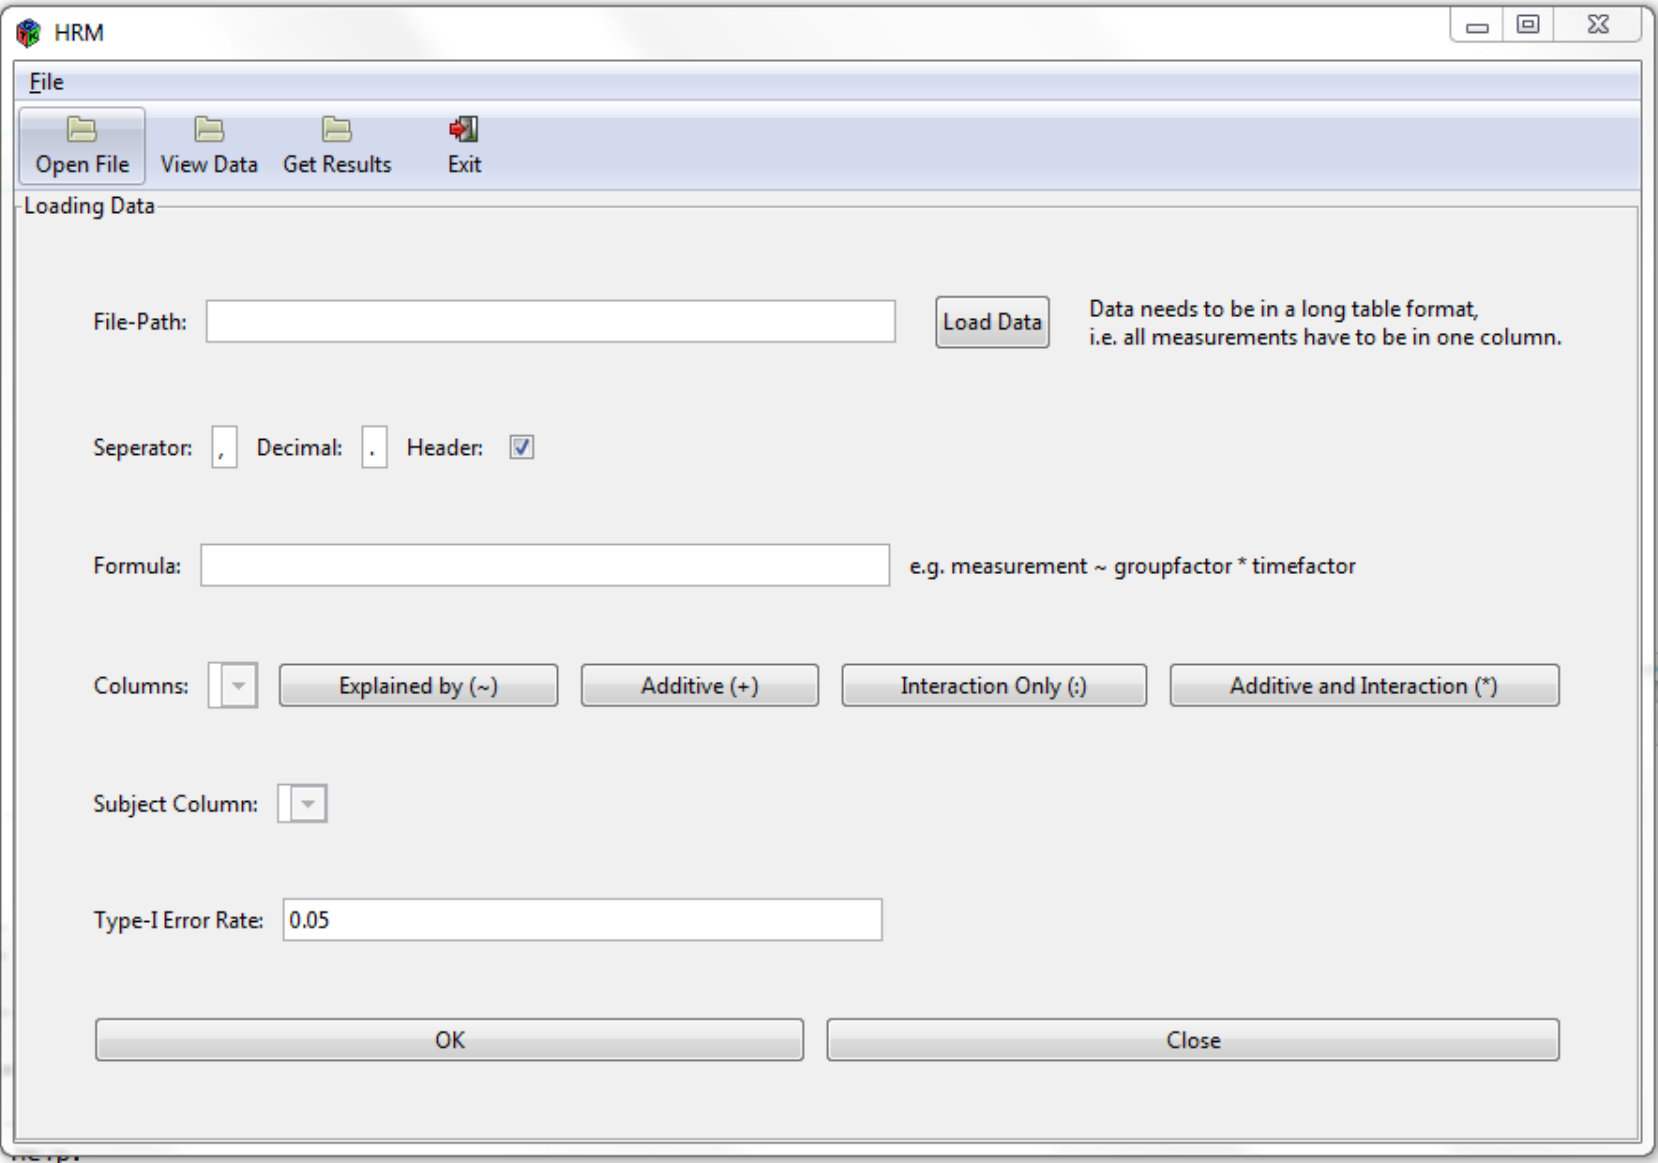
\includegraphics[width=1\textwidth]{GUI}
\includegraphics[width=1\textwidth]{GUI_Two}
\caption{\label{fig:GUI} Base GUI (top) as well as additional GUI for the analysis of two independent samples (bottom). }
\end{figure}
\fi

\subsection{Two independent samples}

As an illustrating example, we use a part of the reaction time data provided by 
\cite{shirley1977non}. In this animal experiment, $N=40$ mice 
were randomized to $a=4$ dose groups ($n=10$ animals per group). The 
observations are the reaction times [in seconds] of mice to stimuli applied to 
their tails. Here, we only use the data from dose group~$0$ (negative control) 
and dose group~$1$ and thus reduce the data set to two independent samples. The 
boxplots of the reaction times as displayed in Figure~\ref{fig:reaction} 
confirm our initial conjecture of quite skewed distributions. 
\begin{figure}[t!]
\centering
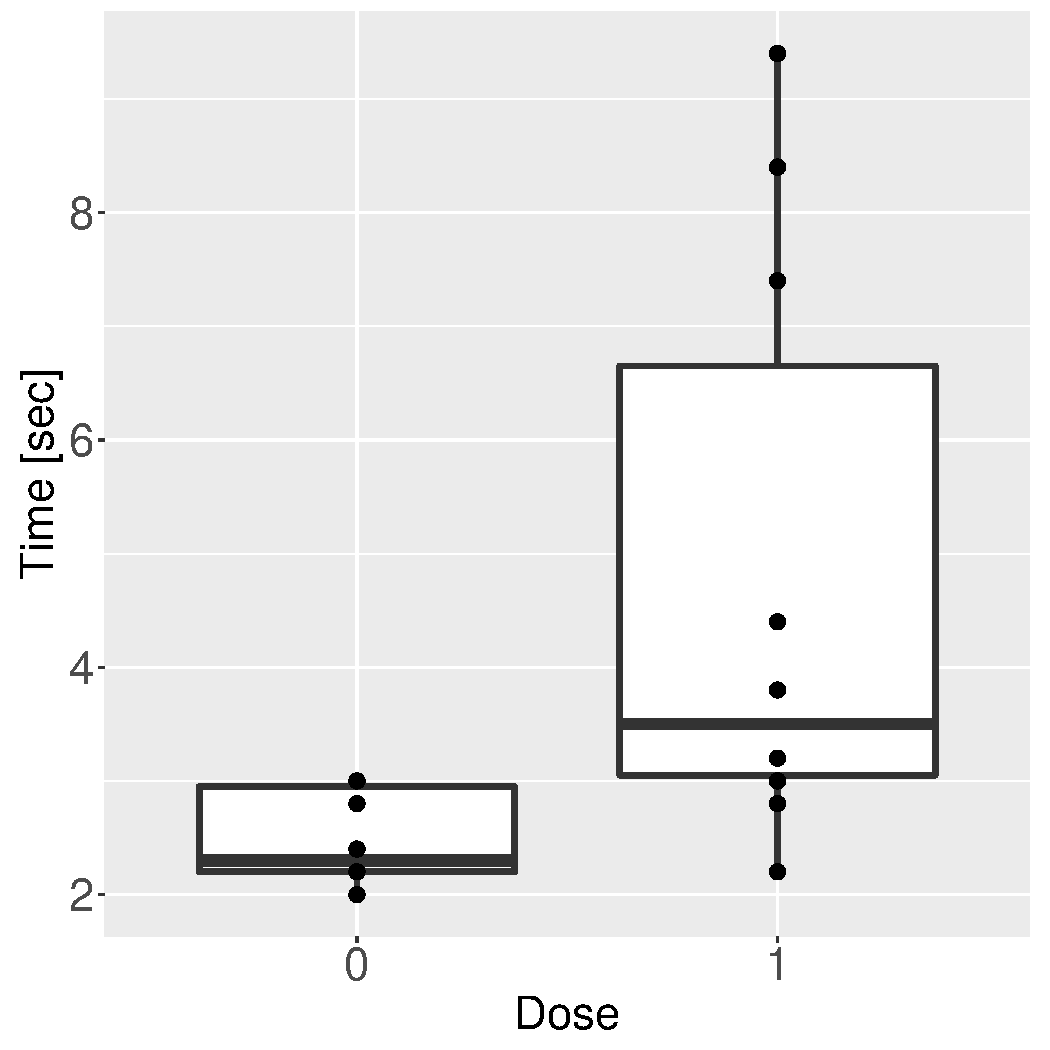
\includegraphics[width=0.47\textwidth]{boxplot_reaction}
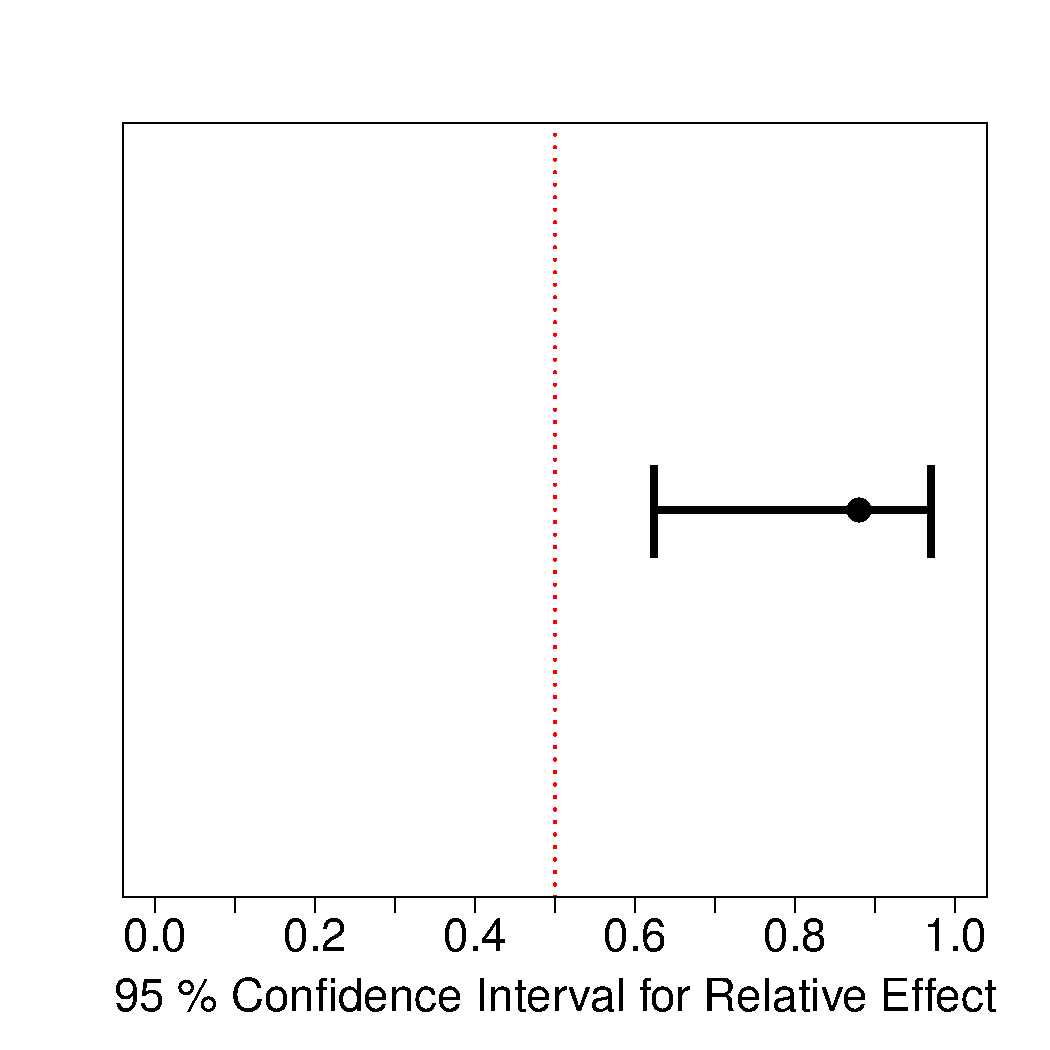
\includegraphics[width=0.52\textwidth]{CI_reaction}
\caption{\label{fig:reaction} Boxplots (left) and 95\%-confidence interval (right) for the relative effect of the reaction time data.}
\end{figure}
In this case, the \emph{Wilcoxon-Mann-Whitney} effect:
\begin{eqnarray*}
\theta=P(X_{01}< X_{11}) +\tfrac12 P(X_{01}=X_{11}),
\end{eqnarray*}
may have a better interpretation for the researcher than the difference of the 
two means. Recall that for 
$\theta<\frac12$ the observations coming from the control group tend to be 
larger than those from group 1. If $\theta=\frac12$, then none of the 
observations tend to be smaller or larger. \textit{No treatment effect} is 
therefore indicated by $\theta=\frac12$. The reaction time data set is 
analyzed with the \fct{rank.two.samples} function. As approximate method, we 
use the \code{logit} approach, compute the \code{exact} 
Wilcoxon-Mann-Whitney test but omit estimation of shift effects:
\begin{example}
library("rankFD")
data("reaction")
\end{example}

%
\begin{example}
A <- rank.two.samples(Time ~ Group, data = reaction, method = "logit",
+                        wilcoxon = "exact", shift.int = FALSE)
\end{example}
\begin{example}
  
               Nonparametric Methods for 2 Independent Samples      
 
 #Alternative: Relative Effect is unequal to 1/2 
 #Method: Logit Transformation 
 #Interpretation: If p(0,1) >1/2, then data in group 1 tend to be 
                  larger than those in group 0 
 #Confidence Level: 95 % 
 #Number of permutations: 10000 
 #Wilcoxon-Mann-Whitney Test: exact 
 #Shift-Effect: NA 
---------------------------------------------------------------------------
Call:
Time ~ Group

Descriptive:
  Sample Size
0      0   10
1      1   10
----------------------Analysis of Relative Effects-------------------------
Test Results:
 Effect Estimator Std.Error      T  Lower  Upper p.Value
 p(0,1)      0.88    0.0801 2.6277 0.6239 0.9701  0.0086

Studentized Permutation Test:
 Effect Estimator Std.Error      T  Lower  Upper p.Value
 p(0,1)      0.88    0.0801 2.6277 0.6551 0.9673  0.0016

-------------------Analysis of Distribution Functions----------------------- 
 
Wilcoxon-Mann-Whitney Test:
 Effect Estimator Statistic p.Value
 p(0,1)      0.88       143  0.0029
\end{example}
\begin{example}
plot(A)
\end{example}

The estimated relative effect $\widehat{\theta}=0.88$ and thus, the estimated 
probability that untreated mice react faster than treated ones is 88\%. 
Furthermore, the data provide the evidence to reject $H_0^\theta: \theta = 
\frac12$ at 5\% level of significance ($p<5\%$) which is also evident in the 
compatible confidence interval (not containing $1/2$).

\subsection{A one-way factorial design}

As an example of a one-way factorial design we use the data set \code{EEG} that 
is included in the package \CRANpkg{MANOVA.RM} 
\citep{friedrich2019manovarm,MANOVARM}. The data set contains EEG measurements 
of 160 patients who were diagnosed with either Alzheimer's Disease (AD), mild 
cognitive impairments (MCI), or subjective cognitive complaints without 
clinically significant deficits (SCC), based on neuropsychological diagnostics 
\citep{bathke2018testing}. For demonstration purposes, we restrict our analysis 
to the measurement of Hjorth complexity (represents change in frequency) obtained at central electrode 
positions. The question of interest is whether this EEG value tends to be larger or smaller than the mean Mann-Whitney effect across the different diseases and therefore, the relative effects defined in (\ref{psiidef})  are used for the analysis. 


\begin{figure}[t!]
	\centering
	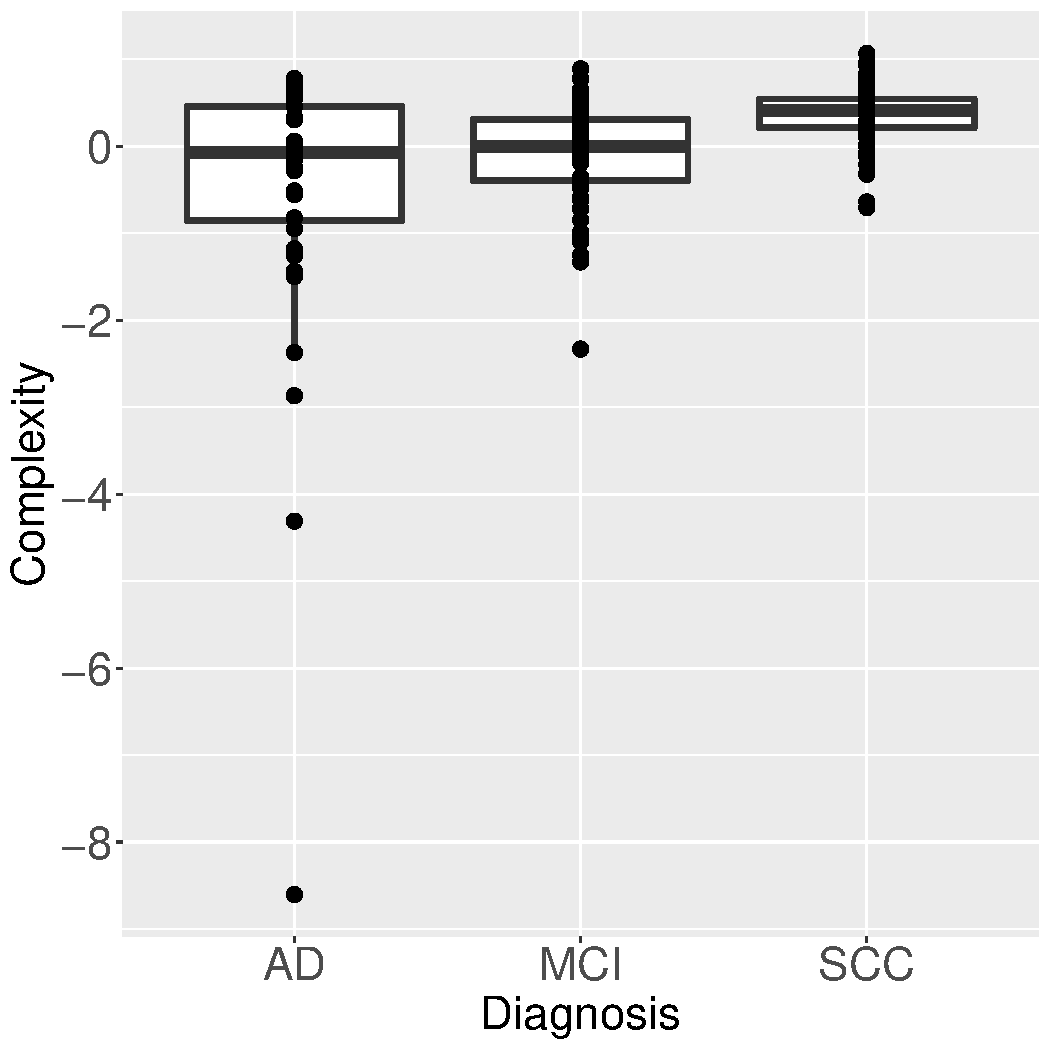
\includegraphics[width=0.47\textwidth]{boxplot_EEG}
		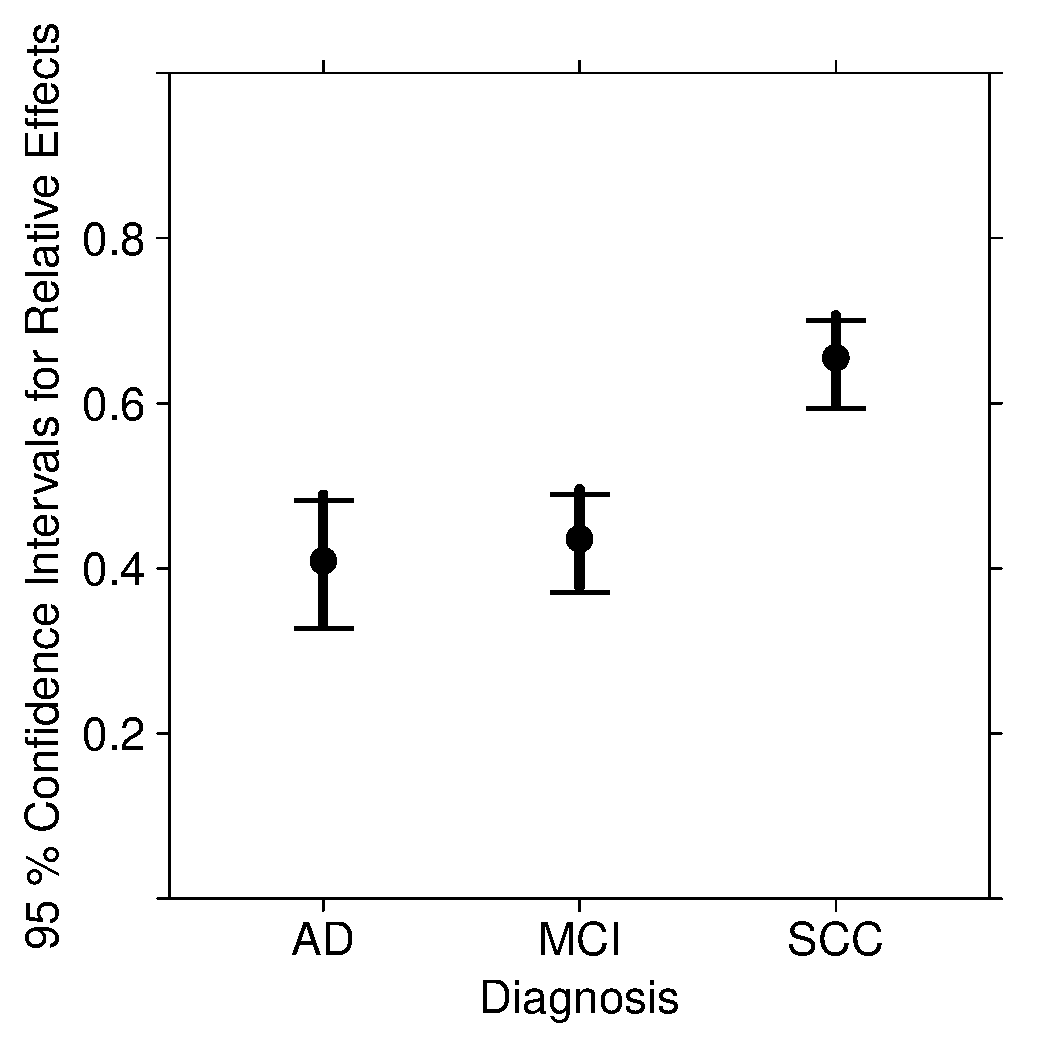
\includegraphics[width=0.49\textwidth]{CI_EEG}
	\caption{\label{fig:EEG} Boxplots (left) and (local) 95\%-confidence intervals for the relative effects of the EEG values (right) .}
\end{figure}



The EEG data is analyzed using the function \fct{rankFD}. Here, we calculate  
confidence intervals with the logit approach and estimate the unweighted relative treatment effects 
to test the null hypothesis $H_0^P$. Moreover, we specify a multiple contrast 
test based on Tukey-type contrasts for the pairwise comparisons of the three 
diagnosis groups.
\begin{example}
library("MANOVA.RM")
data("EEGwide")
B <- rankFD(complexity_central ~ diagnosis, data = EEGwide, 
+	CI.method = "logit", effect = "unweighted", hypothesis = "H0p",
+        contrast = list("diagnosis", "Tukey"))
\end{example}
\begin{example}
		
Nonparametric Methods for General Factorial Designs      

---------------------------------------------------------------------------
#Hypotheses: Tested in Relative Effects 
#Ranking Method: Pseudo-Ranks 
#Confidence Intervals: 95 % with Logit-Transformation 

#MCTP: Fisher Transformation and multivariate T-Approximation
---------------------------------------------------------------------------

Call:
complexity_central ~ diagnosis

Descriptive:
   diagnosis Size Rel.Effect Std.Error  Lower  Upper
1        AD   36     0.4091    0.0400 0.3335 0.4893
2       MCI   57     0.4357    0.0304 0.3773 0.4960
3       SCC   67     0.6551    0.0272 0.6002 0.7063

Wald.Type.Statistic:
          Statistic df p-Value
diagnosis   36.2624  2       0

ANOVA.Type.Statistic:
          Statistic    df1     df2 p-Value
diagnosis   11.1605 1.6222 80.9562   2e-04

MCTP:
$Contrast.Matrix
1  2 3
C1 -1  1 0
C2 -1  0 1
C3  0 -1 1

$Local.Results
  Effect Std.Error      T   Lower  Upper p.value
C1 0.0266    0.0657 0.4044 -0.1308 0.1827  0.9119
C2 0.2460    0.0613 3.8510  0.0941 0.3868  0.0010
C3 0.2194    0.0415 5.1125  0.1176 0.3167  0.0000

$Global.Result
   T0     p.value
1 5.1125       0

$DF
[1] 46

$Quantile
[1] 2.4042
\end{example}
\begin{example}
plot(B)
\end{example}

The output consists of several parts: First, a brief description of the methods 
is given. \code{B\$Descriptive} returns the sample sizes, the estimated relative 
effects as well as their standard errors and confidence intervals for the 
factor levels. \code{B\$ Wald.Type.Statistic} and \code{B\$ANOVA.Type.Statistic} 
return the results of the Wald-type and ANOVA-type test as described in 
Section~\ref{teststat}, respectively. Since we specified our null hypothesis in 
terms of $H_0^P$, Kruskal-Wallis test is not performed. The part \code{B\$MCTP} 
finally contains the results of the multiple contrast test: the contrast matrix 
(Tukey-type), the local test results $T_\ell$ as well as the global results 
$T_0$ along with the $t$-quantile and the corresponding degrees of freedom 
\citep{konietschke2012rank} are reported, see Section~\ref{subsec:MTCP} for 
details. The significant difference between the diagnosis groups and the results of the post-hoc tests reveal that SCC patients differ significantly from the other two 
groups, see also Figure~\ref{fig:EEG}.
%}
%\begin{figure}[t!]
	%\centering
	%\includegraphics{Output_EEG}
	%\caption{\label{fig:EEG_releff} Relative effects and 95 \% confidence 
	% intervals for the EEG values according to diagnosis.}
%\end{figure}


\subsection{A two-way factorial design} 

As an illustrative example of a two-way factorial design, we chose the 
\textit{Irritation of the Nasal Mucosa} trial provided by 
\citet[Chapter~B.3.2]{brunner2019rank} and included in the package. In this trial, the researchers 
investigated the damage of two gaseous substances (factor A) on the nasal 
mucous membrane of mice. Hereby, both substances were given in three different 
concentrations (1[ppm], 2[ppm] and 5[ppm]) (factor B) to 25 mice each. The 
degree of irritation and damage was histopathologically assessed using an 
ordinal score ranging from 0 to 4 with 0 = ``no irritation'', 1 = ``mild 
irritation'', 2 = ``strong irritation'', 3 = ``severe irritation'' and 4 = 
``irreversible damage'', respectively. The outcome is displayed in Figure~\ref{fig:nms}.
\begin{figure}[t!]
	\centering
	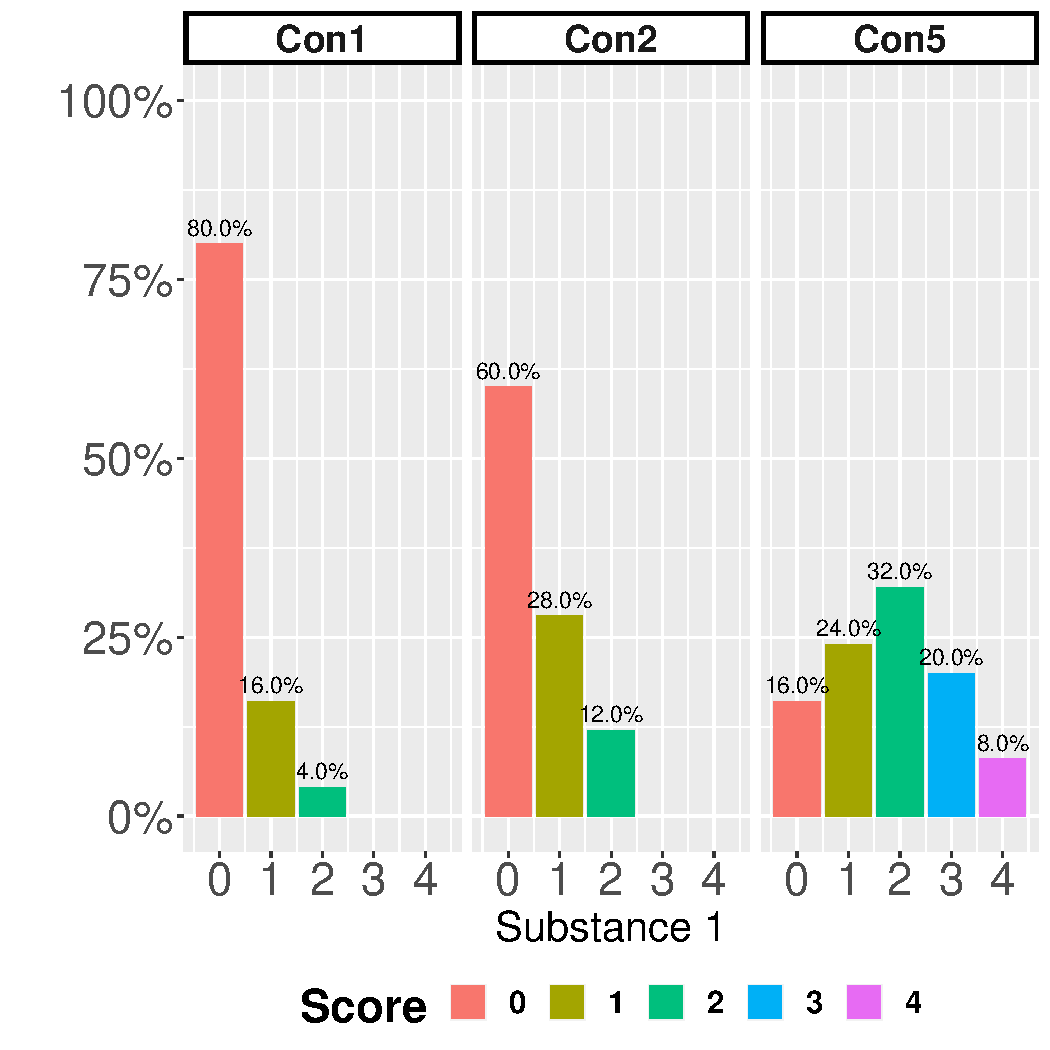
\includegraphics[width=0.47\textwidth]{barplot_nms1}
		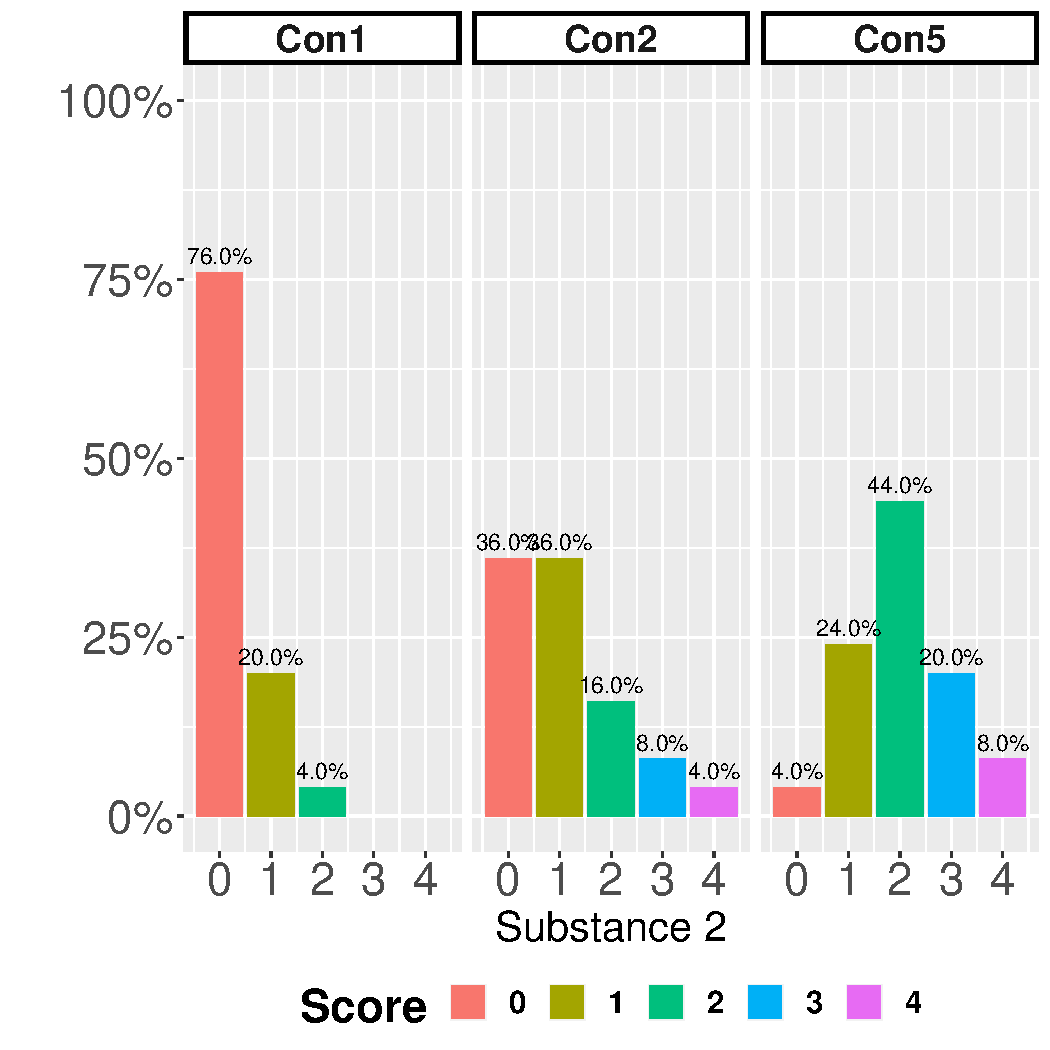
\includegraphics[width=0.47\textwidth]{barplot_nms2}
	\caption{\label{fig:nms} Barplots (percent) of the nasal mucosa scores.}
\end{figure}
The code to analyze this data is similar 
to that provided above, but we additionally include an interaction term in the 
formula. In this example, we formulate  the null hypothesis in terms of the distribution functions to show the R-code for testing this hypothesis. Note that due to the balanced design, both weighted and unweighted estimators give the same results.
\begin{example}
data(nms)	
rankFD(score ~ conc * subst, data = nms, 
+	  hypothesis = "H0F")
\end{example}
\begin{example}

Nonparametric Methods for General Factorial Designs      

---------------------------------------------------------------------------
#Hypotheses: Tested in Distribution Functions 
#Ranking Method: Pseudo-Ranks 
#Confidence Intervals: 95 % with Logit-Transformation 

---------------------------------------------------------------------------

Call:
score ~ conc * subst

Descriptive:
  conc subst Size Rel.Effect Std.Error  Lower  Upper
1    1     1   25     0.3053    0.0310 0.2481 0.3693
2    1     2   25     0.3193    0.0320 0.2601 0.3851
3    2     1   25     0.3927    0.0386 0.3200 0.4704
4    2     2   25     0.5296    0.0459 0.4397 0.6176
5    5     1   25     0.6925    0.0429 0.6027 0.7698
6    5     2   25     0.7605    0.0310 0.6947 0.8159

Wald.Type.Statistic:
            Statistic df p-Value
conc        114.9046  2  0.0000
subst         4.5200  1  0.0335
conc:subst    2.2174  2  0.3300

ANOVA.Type.Statistic:
            Statistic    df1   df2   p-Value
conc         49.8167 1.9289 127.0195  0.0000
subst         4.5200 1.0000 127.0195  0.0354
conc:subst    1.0741 1.9289 127.0195  0.3428


\end{example}
%}

The right plot in Figure~\ref{fig:nmsCI} shows that the relative effects increase at a similar rate in both levels of the main effect suggesting no qualitative interaction between the factor substance and the concentration. 
\begin{figure}[t!]
\centering
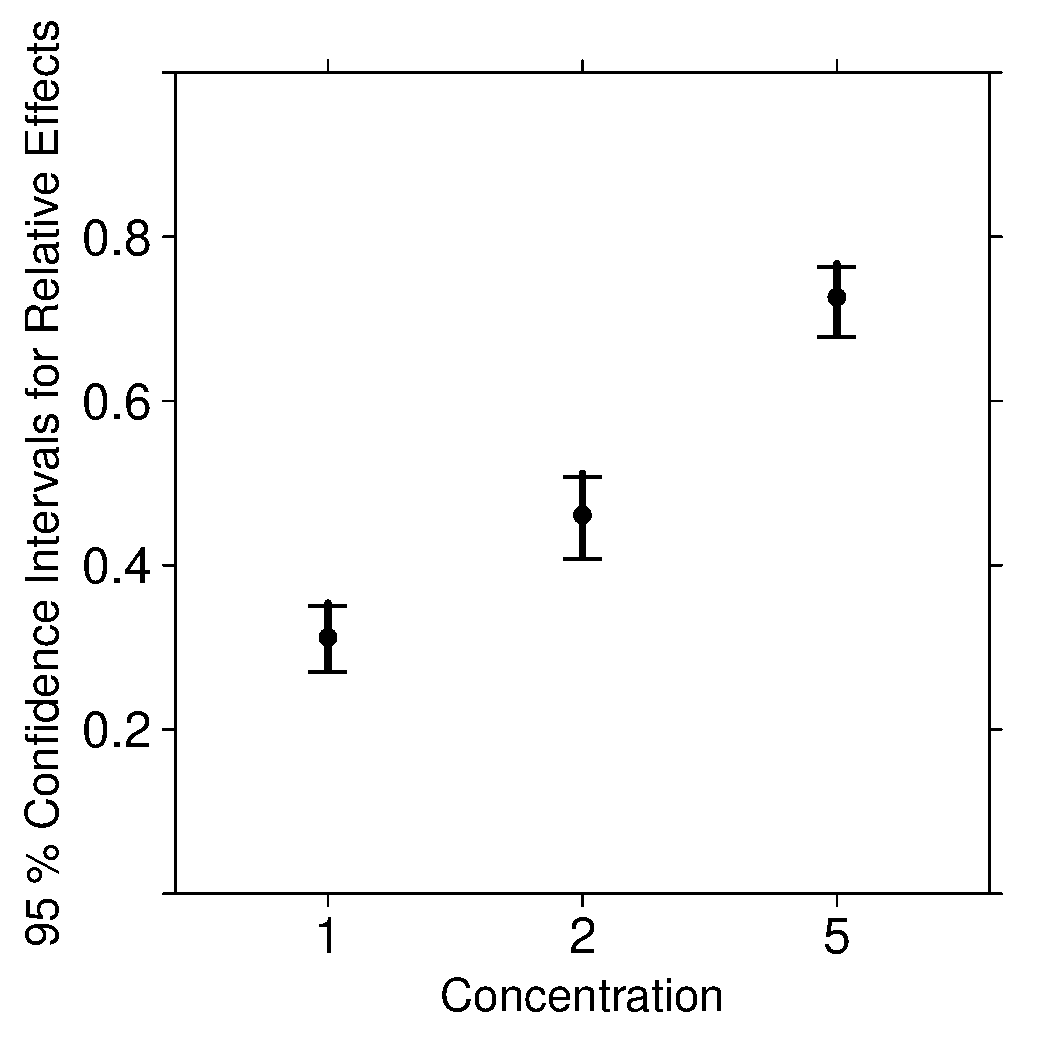
\includegraphics[width=0.32\textwidth]{CI_nms_conc}
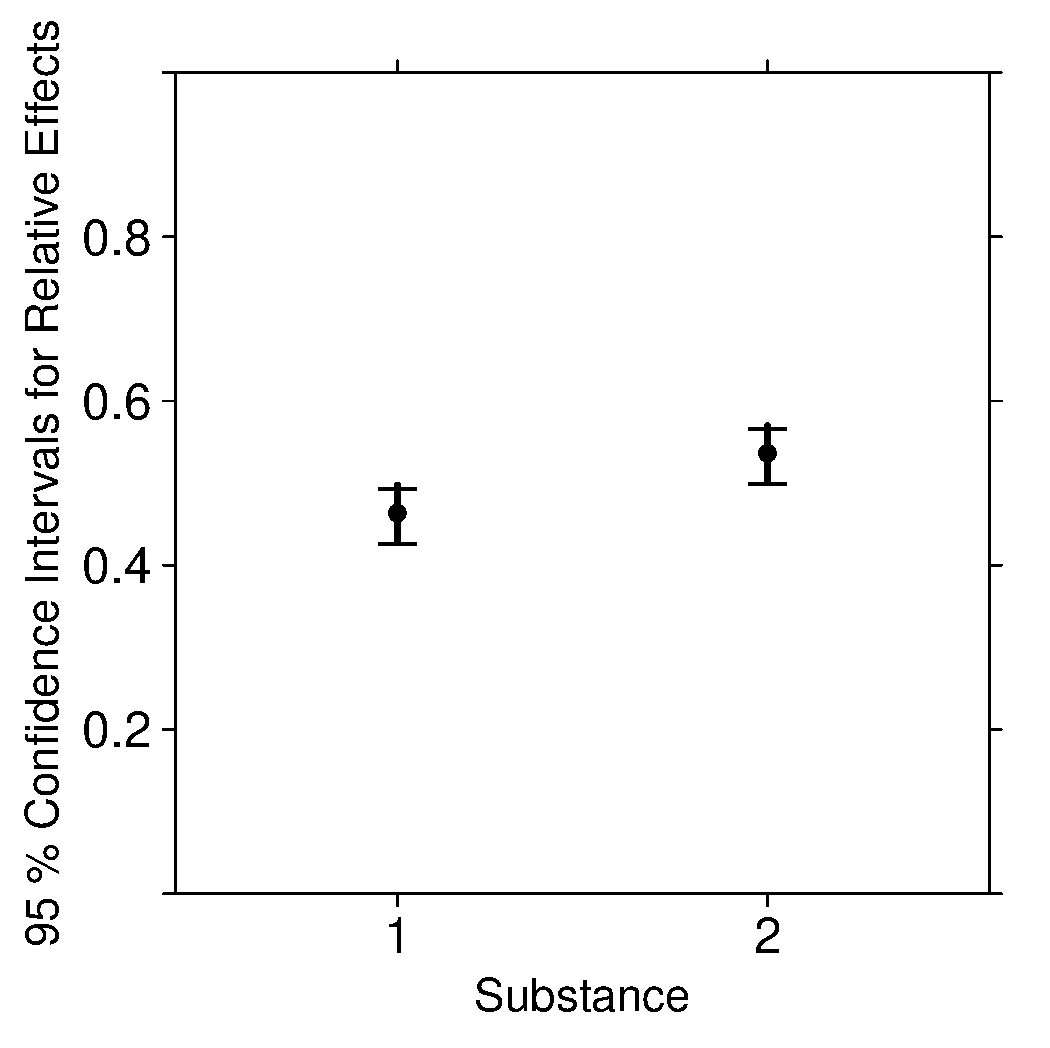
\includegraphics[width=0.32\textwidth]{CI_nms_subst}
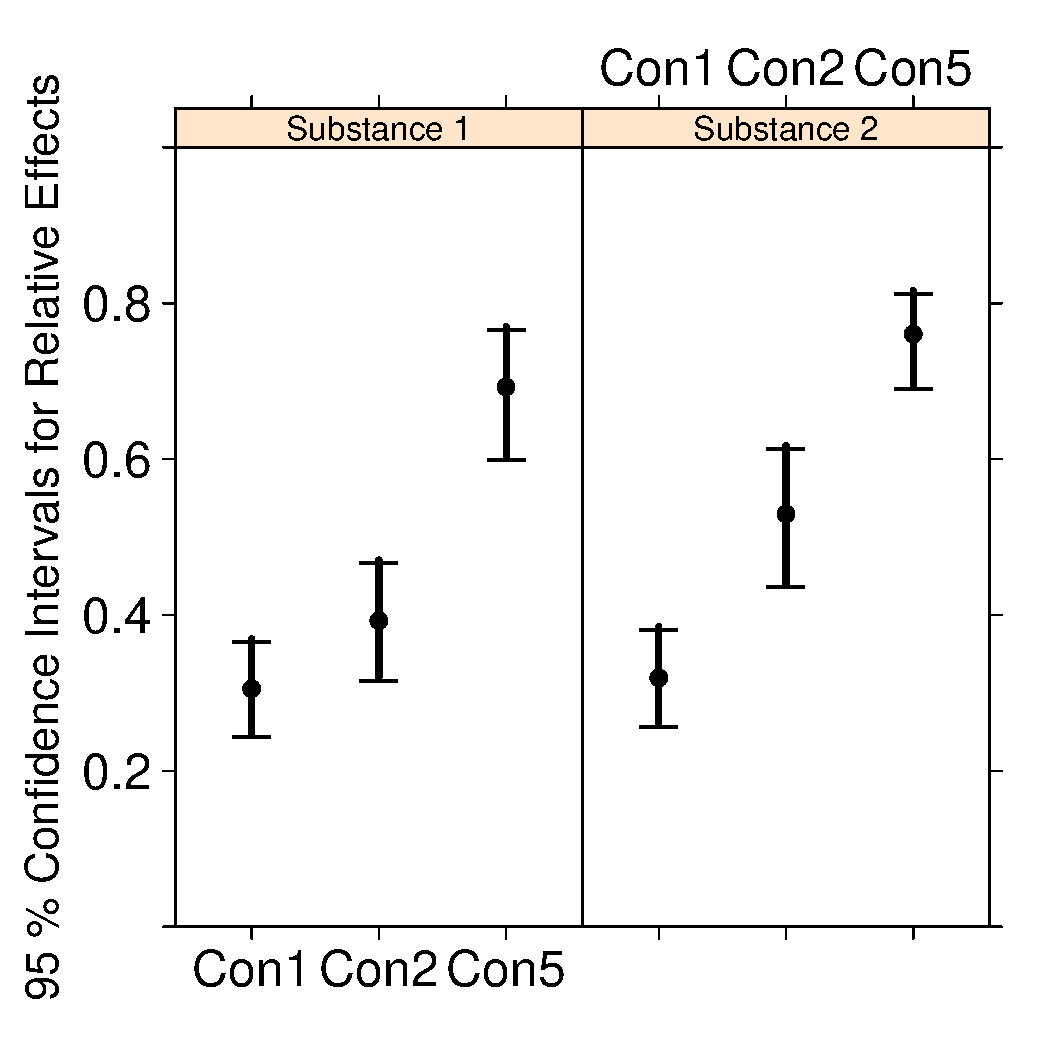
\includegraphics[width=0.32\textwidth]{CI_nms_substconc}
\caption{\label{fig:nmsCI} Local 95\%-confidence interval for the (relative) main and interaction effects of the reaction time data.}
\end{figure}


\section{Summary} \label{sec:summary}
The \CRANpkg{rankFD}-package implements current state of the art rank methods for nonparametric
inference in general factorial designs with independent observations. It comprises of functions for computing various test statistics for testing null hypotheses formulated either in distribution functions
or in relative effects using ranks or  pseudo-ranks, respectively. Up until now, no other software package for testing null hypotheses in relative effects in general factorial designs have existed.  Besides global procedures (Wald-type and ANOVA-type statistics) using quadratic forms, \CRANpkg{rankFD} implements multiple contrast tests  and simultaneous confidence intervals for relative effects. The possibility of testing contrasts between the main and interaction effects makes \CRANpkg{rankFD} a powerful tool for the application of nonparametric methods in data analysis and a useful addition to \CRANpkg{nparcomp} \citep{konietschke2015nparcomp}. Besides the inference methods discussed above, \CRANpkg{rankFD} furthermore implements formulas for computing sample sizes using the functions \fct{WMWSSP} and \fct{noether} \citep{happ2019optimal}. Since these methods apply for two independent samples only, we did not discuss them in the present manuscript. %Furthermore, a GUI facilitates the command driven use of its functions, which makes the software very user-friendly, especially if it is used in teaching purposes.

We designed the package and its functions to be similar to the well known \textit{R}-functions \fct{lm}, \fct{aov} for the analysis of linear models and the \fct{glht} function of the \CRANpkg{multcomp} package for the computation of multiple contrast tests in means. Both \CRANpkg{rankFD} and \CRANpkg{multcomp} use the \CRANpkg{mvtnorm} package \citep{genz2021package} for the computation of critical values. However, as explained in detail in the Introduction, the effect measures used in multcomp and mvtnorm are different from those used in \CRANpkg{rankFD}. In general parlance, this means that the parametric and nonparametric methods are not comparable at hand. 

  
We plan to update \CRANpkg{rankFD} frequently with novel procedures. For instance, various international research groups are currently investigating rank-based methods for the analysis of clustered data, see also the package \CRANpkg{clusrank} \cite{jiang2017wilcoxon} for the analysis of two samples, sample size planning, as well as analysis of covariance methods. We plan to add these methods in the future. The package \CRANpkg{rankFD} is online available
on \textit{CRAN}. \\

\textbf{Acknowledgement:} The authors are grateful to the Editor and two anonymous referees
for helpful comments which considerably improved the paper. This work was
supported by the German Research Foundation project DFG KO 4680/4-1.

   




%% -- Optional special unnumbered sections -------------------------------------





\bibliography{rankFD_FINAL}




\address{Frank Konietschke\\
Charit\'e Universit\"atsmedizin Berlin\\
Institute of Biometry and Clinical Epidemiology\\
Reinhardstr. 58\\
10117 Berlin, Germany\\
\email{Frank.Konietschke@charite.de}}

\address{Edgar Brunner\\
  University Medical School G\"ottingen\\
  Institut f\"ur Medizinische Statistik\\
  Humboldtallee 32\\
	37073 G\"ottingen, Germany\\
  \email{ebrunne1@gwdg.de}}

\end{article}

\end{document}
